\documentclass[border=10pt]{standalone}

\usepackage{tikz}
\usepackage{tikzsymbols}
\usetikzlibrary{calc,patterns,shapes.geometric}

\def\centerarc[#1](#2)(#3:#4:#5){\draw[#1] ($(#2)+({#5*cos(#3)},{#5*sin(#3)})$) arc (#3:#4:#5);}

\begin{document}
	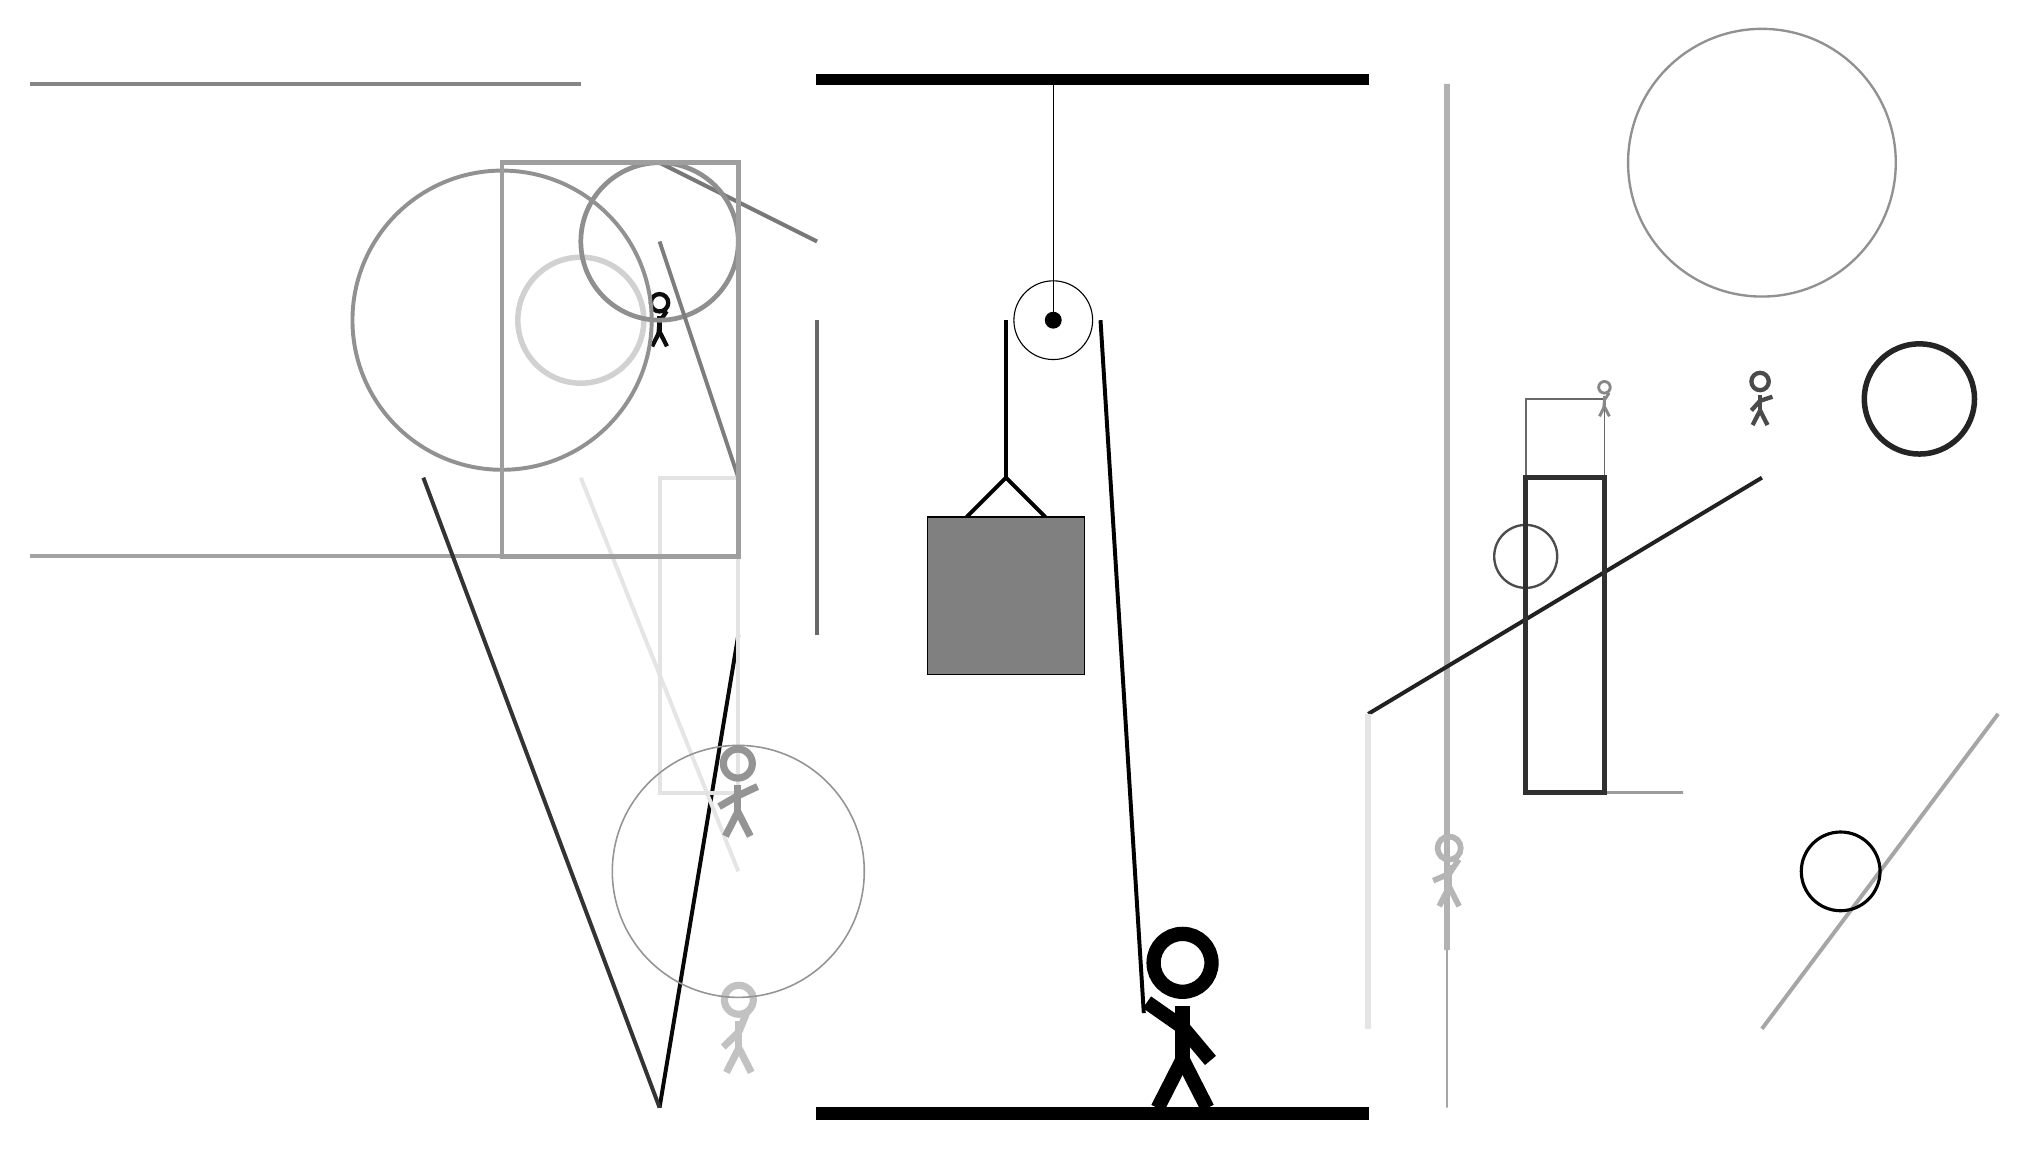
\begin{tikzpicture}
		%%%%% START %%%%%
		
		\draw[fill=black] (-2, 10) rectangle (5, 10.125);
		
		\draw (1, 7) circle (0.5);
		\draw[fill=black] (1, 7) circle (0.1);
		\draw (1, 10) -- (1, 7);
		
		\draw[line width=0.5mm] (-0.1, 4.5) -- (0.4, 5.0) -- (0.9, 4.5);
		\draw[fill=black!50] (-0.6, 4.5) rectangle (1.4, 2.5);
		
		\draw[line width=0.5mm] (0.4, 7) -- (0.4, 5.0);
		\centerarc[line width=0.5mm](1, 7)(0:180:0.6);
		\draw[line width=0.5mm](1.6, 7) -- (2.15, -1.8);
		
		\node at (2.6, -1.9) {\Strichmaxerl[10][-35][-50]};
		
		\draw [line width=0.7mm, color=black!18](-5, 7) circle (0.8);
		
		\draw[line width=0.2mm, color=black!59] (7, 1) rectangle (8, 6);
		\draw [line width=0.3mm, color=black!30](-4, -3) circle (0.0);
		\node[line width=0.2mm, color=black!71] at (10, 6) {\Strichmaxerl[3][48][18]};
		\draw[line width=0.5mm, color=black!97](-4, -3) -- (-3, 3);
		\draw [line width=0.7mm, color=black!86](12, 6) circle (0.7);
		\draw [line width=0.3mm, color=black!70](7, 4) circle (0.4);
		\node[line width=0.6mm, color=black!95] at (-4, 7) {\Strichmaxerl[3][85][57]};
		\draw[line width=0.5mm, color=black!59](-2, 3) -- (-2, 7);
		\draw[line width=0.5mm, color=black!36](-4, 4) -- (-12, 4);
		\draw[line width=0.7mm, color=black!30] (6, -1) rectangle (6, 10);
		\node[line width=0.3mm, color=black!24] at (-3, -2) {\Strichmaxerl[5][44][68]};
		\draw[line width=0.2mm, color=black!35] (6, -1) rectangle (6, -3);
		\draw[line width=0.4mm, color=black!39] (7, 1) rectangle (9, 1);
		\draw[line width=0.5mm, color=black!87](10, 5) -- (5, 2);
		\draw[line width=0.5mm, color=black!35](10, -2) -- (13, 2);
		
		\draw[line width=0.5mm, color=black!10](-3, 0) -- (-5, 5);
		\draw [line width=0.4mm, color=black!100](11, 0) circle (0.5);
		\draw[line width=0.3mm, color=black!74] (-2, 9) rectangle (-2, 9);
		\draw[line width=0.5mm, color=black!53](-2, 8) -- (-4, 9);
		\node[line width=0.7mm, color=black!47] at (8, 6) {\Strichmaxerl[2][85][57]};
		
		\draw [line width=0.3mm, color=black!43](10, 9) circle (1.7);
		
		\draw[line width=0.5mm, color=black!11] (-3, 5) rectangle (-4, 1);
		\draw[line width=0.7mm, color=black!81] (7, 5) rectangle (8, 1);
		\node[line width=0.2mm, color=black!42] at (-3, 1) {\Strichmaxerl[5][30][25]};
		
		\draw[line width=0.7mm, color=black!10] (5, 2) rectangle (5, -2);
		\draw[line width=0.5mm, color=black!48](-5, 10) -- (-12, 10);
		\draw [line width=0.2mm, color=black!42](-3, 0) circle (1.6);
		\draw [line width=0.6mm, color=black!44](-4, 8) circle (1.0);
		\draw [line width=0.5mm, color=black!43](-6, 7) circle (1.9);
		\draw[line width=0.5mm, color=black!51](-4, 8) -- (-3, 5);
		
		\node[line width=0.6mm, color=black!29] at (6, 0) {\Strichmaxerl[4][23][56]};
		\draw[line width=0.6mm, color=black!38] (-3, 4) rectangle (-6, 9);
		\draw[line width=0.5mm, color=black!80](-4, -3) -- (-7, 5);
		
		
		\draw[fill=black] (-2, -3) rectangle (5, -3.15);
		
		%%%%% END %%%%%
	\end{tikzpicture}
\end{document}